\section{Patientgruppe}
\textit{Følgende afsnit omhandler omfanget af lidelsen, knæartrose. Afsnittet redegør for patientomfanget, samt de forskellige disponeringsfaktorer sammenkoblet med lidelsen. Ydermere vil patienternes patientforløb blive redegjort, hvoraf den sidste fase vil blive analyseret. Ovenstående vil danne grundlag for at klassificere en patientgruppe til knæalloplastik.}

Knæartrose er en lidelse der gradvist nedbryder knæets ledbrusk, hvorefter der kan forekomme forandringer i leddets knogler og slimhinder. Disse deformationer er irreversible, hvormed knæartrose kun kan afhjælpes og ikke kurreres. Lidelsen kan opdeles i en primær- og sekundær artrose. Den primære artrose er bestående af ikke-udefrakommende årsager, hvilket indebærer genetik samt aldring. Den sekundære artrose indebærer tidligere skader, sygdom, inflammation, overvægt samt traume. Knæartrose er en tilstand hvis hyppigste symptomer er smerter, nedsat mobilitet samt fejlstilling af leddet hos den påvirkede. Smerterne udtrykkes i forskellig grad, fra igangsættende smerte til kronisk tilstedeværende smerte. Generelt for knæartrose, forværres symptomerne i takt med graden af lidelsen øges. \citep{Lind2016b}

En længere række faktorer har betydning for udviklingen af artrose. Hvis en eller flere af disse faktorer er tilstede, er den påvirkede mere disponeret for knæartrose. Dette er eksempelvis, overbelastning igennem arbejde og fritid, tidligere knæskader, genetisk arv, overvægt samt køn \citep{brostrom2012}. Knæartrose er til stede blandt 45\% af alle 80-årige i befolkningen. Antallet af personer med knæartose kan formodes at stige da levealderen i Danmark stiger. Dette er ikke det eneste faktor, hvorfor prævalensen kan antages at stige. En af risikofaktorerne for udviklingen af knæartrose er overvægt, hvilket 47\% af den danske befolkning kan kategoriseres som. Ydermere stiger andelen af overvægtige med alderen, hvilket ligeledes er tilfældet for knæartrose. Overvægtige med en høj body-mass-index (BMI) er disponeret for knæartrose med en relativ risiko på en faktor tre, hvoraf en kombination af ovenstående faktorer øger risikoen for lidelsen. Dog kan der opstå problematikker vedrørende benyttelsen af BMI, da metoden ikke skelner mellem fedt og muskler. \textbf{(8)} \citep{brostrom2012} \citep{Vestergaard2014} \citep{Vestergaard2016} \citep{Lind2016} \citep{Lind2016b}

En patients symptomer kan medføre igangsættelsen af et behandlingsforløb. Et behandlingsforløb for en patient med knæartrose består af flere faser, hvis mål er smertelindring, mobilitetsforøgelse samt forebyggelse. Generelt kan faserne opdeles i ikke-invasive og invasive metoder. Hvilken metode som hjælper patienten afhænger af graden af knæartrose.

\begin{figure}[H]
	\centering
	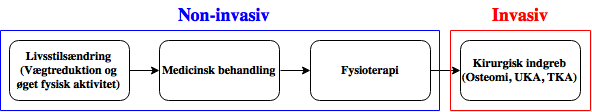
\includegraphics[width=1\textwidth]{figures/bProblemanalyse/flowchart_behandlingsforloeb.png}
	\caption{På figuren ses et flowchart indeholdende de forskellige behandlingsmetoder der forekommer igennem et patientforløb med knæartrose.}
	\label{fig:flow_behandlingsfaser}
\end{figure}\vspace{-.25cm}

Som det ses på \figref{fig:flow_behandlingsfaser}, består første fase, hvis nødvendig, af en livsstilsændring, hvor en vægtreduktion samt øget fysisk aktivitet uden belastning, kan afhjælpe patients symptomer. Hvis dette ikke er tilstrækkeligt kan medicinsk behandling i form af smertelindrende medikamenter benyttes, enten som enkeltstående behandling eller sideløbende med fysioterapi. Hvis ikke, de non-invasive behandlingsmetoder afhjælper lidelsen i en grad hvor patienten er tilfreds, så bliver de invasive behandlingsmetoder taget til overvejelse. Overvejelsen heraf indebærer den diagnosticerede grad af artrose, hvilket består af en sammenkobling af den kliniske vurdering, verificeret med forandringer i knæet opnået gennem røntgenbilleder. Baggrunden for at den kliniske vurdering skal verificeres forud for kirurgi, er at smerte fra hofte og ryg, kan projiceres til knæet. Resultatet heraf er at patienten først berettiget kirurgi og hermed en total knæalloplastik (TKA), når non-invasive behandlingsmetoder ikke har kunne afhjælpe problemet til en grad med overkommelige symptomer(\textbf{4}). Ydermere skal patienten besidde moderat til svær artrose for at kunne kvalificeres til kirurgi. \citep{Lind2016b} \citep{brostrom2012} \citep{skou2016}

En TKA operation er den sidst mulige behandlingsmetode for at lindre patientens symptomer vedrørende knæartrose. Dette resulterede i at der i 2014 blev udført omtrent 9.800 TKA operationer, fordelt på førstegangs- og revisions operationer. \citep{aarsrapport2016} Idet TKA operationen er den sidste behandlingsmulighed, er operationstilfredshed en betydningsfuld problematik. I 2012 viste en undersøgelse fra Sundhedsstyrelsen, at 81-85\% af patienter der havde modtaget en TKA operation var tilfredse, 8-11\% var decideret utilfredse, og resten var i tvivl eller til dels utilfreds. Dette er ensbetydende med at der potentielt er 19\% af alle operationer fra et patientøjemed som ikke er succesfulde. Resultatet heraf er at op mod 19\% ikke opnår bedring fra deres smerter samt eventuel nedsat mobilitet. \citep{brostrom2012} Sundhedsstyrelsens indikationer vedrørende patientutilfredshed er entydig med flere studier omhandlende samme emne på internationalt plan. Dette understøttes blandt andet i studiet af \cite{Bourne2010}, som ligeledes har opnået resultater, der indikerer at 19\% er utilfredse med deres TKA operation. Studiet har ydermere undersøgt den generelle tendens omhandlende utilfredshed, hvilket befinder sig i området 25-11\% (Se \tabref{tab:patient_utilfreds}). \citep{Bourne2010} Det påpeges ydermere i et studiet af \cite{Jacobs2014} at hverken alder, køn eller BMI, havde indflydelse på hvilke af patienterne der var utilfredse. \citep{Jacobs2014}   \textbf{(5)}
\begin{table}[H]
	\centering
\begin{tabular}{ccc}
	\hline
	\rowcolor[HTML]{C0C0C0} 
	Studie            & Forsøgspopulation {[}N{]} & Utilfreds {[}\%{]} \\ \hline
	Anderson et al.   & 74                        & 11                 \\
	Noble et al.      & 253                       & 25                 \\
	Robertsson et al. & 27.372                    & 18                 \\
	Wylde et al.      & 228                       & 15                 \\
	Hawker et al.     & 1193                      & 15                 \\
	Heck et al.       & 291                       & 12                 \\
	Bourne et al.     & 1703                      & 19                 \\ \hline
\end{tabular}
	\caption{I tabellen ses \cite{Bourne2010} sammenligning af flere studiers resultater vedrørende patientutilfredshed efterfulgt en TKA operation. \citep{Bourne2010}}
	\label{tab:patient_utilfreds}
\end{table}

\cite{Sakellariou2016} har lavet en risikovurdering vedrørende kroniske smerter efter en TKA operation. Udfra resultaterne viste \cite{Sakellariou2016}, at op mod 39\% af studiets patienter oplevede moderat til alvorlig smerte, et år postoperativt TKA. Dog kan der ikke drages en parallel mellem smerte og ovennævnte utilfredshed. Dette er tilfældet da det kan forestilles at den kroniske smerte stadig kan være en forbedring, hvilket resultaterne omhandlende utilfredshed også indikerer. Indikationen heraf ses, da ingen resultater vedrørende utilfredshed er i omegnen af 39\%. \textbf{(6 1:2)} \citep{Sakellariou2016} I studiet af \cite{Jacobs2014} var størstedelen af forsøgspopulationens utilfredshed relateret til enten passiv fleksion, smerte eller funktion, sammenholdt med præoperative test. Resultaterne fra de præoperative test indikerede at der ikke var signifikant forskel vedrørende smerte eller funktion, blandt de tilfredse og de utilfredse patienter. Postoperativt blev samme test udført, og her var der signifikant forskel ved alle indikationer, passiv fleksion, smerte og funktion. Den utilfredse gruppe havde opnået signifikant dårligere resultater, hvormed dette kan antages som værende grunden til patienternes utilfredshed. \citep{Jacobs2014} Dette fund understøttes ligeledes af studiet af \cite{Bourne2010}, hvis resultater indikerer at de utilfredse patienter har signifikant flere smerter, led stivhed samt nedsat funktion et år efter operationen, sammenholdt med de tilfredse patienter. \citep{Bourne2010} \textbf{(6 2:2)}  

Patientgruppen som postoperativt ikke er tilfredse er svært definerbar. Problematikken opstår i og med klassificeringen bag de potentielt 11 til 25~\% utilfredse patienter er vedrørende postoperative smerte samt funktion. Det kan forestilles at der blandt nogle af patienterne findes en forventningsfaktor, hvilket gør de kategoriserer sig selv som værende utilfreds, omend de rent faktisk har opnået en forbedring af både smerte og eller mobilitet. Det kan tænkes at forventningsfaktoren kan være medvirkende til at kategorisere dem som værende utilfredse, som resultat af skuffelsen af ikke at fungere som et individ med et fuldt funktionsdygtigt knæ. Denne antagelse understøttes af \cite{Bourne2010}, som beskriver de største prædiktorer omhandlende utilfredshed efterfulgt af en TKA operation. Den faktor som besidder den største score er, patientens forventninger til operationen ikke er mødt, hvilket medfører 10,7 gange større risiko for utilfredshed. \citep{Bourne2010} I et andet studie af \cite{Keudell2013} bliver patienternes alder sammenkoblet med deres forventninger. Det tyder på at den ældre patientgruppe (>65 år) har generelt har lavere forventninger til operationsresultatet, end den yngre patientgruppe (<55 år). I dette studie indikeres det at den ældre patientgruppe generelt har større tilfredshed, end den yngre. Dette kan antages at have en sammenhæng med påstanden fra \cite{Bourne2010}, vedrørende prædiktoren til utilfredshed, omhandlende forventninger til operationen. \textbf{(7 (mangler analyse?))}

Knæartrose er en lidelse i vækst da den umiddelbare disponerede målgruppe er voksende. Resultatet heraf medfører at antallet af registrerede tilfælde med symptomer sandsynligvis ligeledes vil stige, og der i fremtiden vil blive udført flere operationer, hvoraf det kan antages at der vil forekomme flere patienter med kroniske smerter postoperativt TKA, uden mulighed for yderligere behandling.

